\chapter{Uvod}
\label{ch:uvod}

%Cilj magistrske naloge je pripraviti simulator STG stroja, nato pa spremeniti STG jezik tako, da bo namesto avtomatičnega čistilca pomnilnika uporabljal model lastništva po zgledu programskega jezika Rust. Zanimalo nas bo, kakšne posledice to v STG stroj prinese, kakšne omejitve se pri tem pojavijo ter do kakšnih problemov lahko pri tem pride. Zavedati se moramo, da obstaja možnost, da koncepta lastništva ni mogoče vpeljati v STG stroj brez korenitih sprememb zasnove stroja samega - v tem primeru bomo podali analizo, zakaj lastništva v STG stroj ni mogoče vpeljati.

\section{Upravljanje s pomnilnikom}

% V magistrskem delu se bomo primarno ukvarjali s STG jezikom. Operacijska semantika tega veleva, da so vsi izrazi v izvorni kodi v pomnilniku predstavljeni kot zaprtja. Jezik vsebuje izraz \texttt{let}, ki na kopici ustvari novo zaprtje, izbirni izraz \texttt{case} pa šele dejansko izračuna njegovo vrednost. Jezik STG za čiščenje zaprtij iz kopice uporablja generacijski čistilec pomnilnika~\cite{jones1992implementing, marlow2004making}. 

% Cilj magistrske naloge je pripraviti simulator STG stroja, nato pa spremeniti STG jezik tako, da bo namesto avtomatičnega čistilca pomnilnika uporabljal model lastništva po zgledu programskega jezika Rust. Zanimalo nas bo, kakšne posledice to v STG stroj prinese, kakšne omejitve se pri tem pojavijo ter do kakšnih problemov lahko pri tem pride. Zavedati se moramo, da obstaja možnost, da koncepta lastništva ni mogoče vpeljati v STG stroj brez korenitih sprememb zasnove stroja samega - v tem primeru bomo podali analizo, zakaj lastništva v STG stroj ni mogoče vpeljati.

Pomnilnik je dandanes kljub uvedbi pomnilniške hierarhije še vedno eden izmed najpočasnejših delov računalniške arhitekture. Učinkovito upravljanje s pomnilnikom je torej ključnega pomena za učinkovito izvajanje programov. Upravljanje s pomnilnikom v grobem ločimo na ročno in avtomatično~\cite{jones2023garbage}. Pri ročnem upravljanju s pomnilnikom programski jezik vsebuje konstrukte za dodeljevanje in sproščanje pomnilnika. Odgovornost upravljanja s pomnilnikom leži na programerju, zato je ta metoda podvržena človeški napaki. Pogosti napaki sta puščanje pomnilnika (angl. memory leaking), pri kateri dodeljen pomnilnik ni sproščen, in viseči kazalci (angl. dangling pointers), ki kažejo na že sproščene in zato neveljavne dele pomnilnika~\cite{jones2023garbage}.

Pri ročnem upravljanju pomnilnika kot ga poznamo npr. pri programskem jeziku C, pride pogosto do dveh vrst napak~\cite{jones2023garbage}:

\begin{itemize}
	\itemsep 0em
	\item viseči kazalci (angl. dangling pointers) so kazalci na pomnilnik, ki je že bil sproščen.
	\item puščanje pomnilnika (angl. memory leak), 
	\item uporaba po sproščanju (angl. use-after-free), pri kateri skušamo dostopati do pomnilnika, ki je bil že prej sproščen in
	\item dvojno sproščanje (angl. double free), pri katerem skušamo dvakrat sprostiti isti pomnilniški naslov.
\end{itemize}

V obeh primerih bo prišlo do nedefiniranega obnašanja sistema za upravljanje s pomnilnikom (angl. memory management system). Ob uporabi po sproščanju lahko pride npr. do dostopanja do pomnilniškega naslova, ki ni več v lasti trenutnega procesa in posledično do sesutja programa. V primeru dvojnega sproščanja pa lahko pride do okvare delovanja sistema za upravljanje s pomnilnikom, kar lahko privede do dodeljevanja napačnih naslovov ali prepisovanja obstoječih podatkov na pomnilniku.

Druga možnost upravljanje s pomnilnikom je avtomatično upravljanje pomnilnika, pri katerem zna sistem sam dodeljevati in sproščati pomnilnik. Tukaj ločimo posredne in neposredne metode.

Ena izmed neposrednih metod je npr. štetje referenc~\cite{collins1960method}, pri kateri za vsak objekt na kopici hranimo metapodatek o številu kazalcev, ki se sklicujejo nanj. V tem primeru moramo ob vsakem spreminjanju referenc zagotavljati še ustrezno posodabljanje števcev, kadar pa število kazalcev pade na nič, objekt izbrišemo iz pomnilnika. Ena izmed slabosti štetja referenc je, da mora sistem ob vsakem prirejanju v spremenljivke posodobiti še števce v pomnilniku, kar privede do povečanja števila pomnilniških dostopov. Prav tako pa metoda ne deluje v primeru pomnilniških ciklov, saj števec referenc nikoli ne pade na nič, kar pomeni da pomnilnik nikoli ni ustrezno počiščen.

Posredne metode, npr. označi in pometi~\cite{mccarthy1960recursive}, ne posodabljajo metapodatkov na pomnilniku ob vsaki spremembi, temveč se izvedejo le, kadar se prekorači velikost kopice. Algoritem pregleda kopico in ugotovi, na katere objekte ne kaže več noben kazalec ter jih odstrani. Nekateri algoritmi podatke na kopici tudi defragmentirajo in s tem zagotovijo boljšo lokalnost ter s tem boljše predpomnjenje~\cite{fenichel1969lisp}. Problem metode označi in pometi pa je njeno nedeterministično izvajanje, saj programer oziroma sistem ne moreta predvideti kdaj se bo izvajanje glavnega programa zaustavilo in tako ni primerna za časovno-kritične (angl. real-time) aplikacije.

% Avtomatično čiščenje pomnilnika pa ima tudi svoje probleme. Štetje referenc v primeru pomnilniških ciklov privede do puščanja pomnilnika, metoda označi in pometi pa nedeterministično zaustavi izvajanje glavnega programa in tako ni primerna za časovno-kritične (angl. real-time) aplikacije. Kot alternativa obem načinom upravljanja s pomnilnikom sistemski programski jezik Rust implementira model lastništva~\cite{klabnik2023rust}. Med \textit{prevajanjem} zna s posebnimi pravili zagotoviti, da se pomnilnik objektov na kopici avtomatično sprosti, kadar jih program več ne potrebuje. To pa zna storiti brez čistilca pomnilnika in brez eksplicitnega dodeljevanja in sproščanja pomnilnika, zato zagotavlja predvidljivo sproščanje pomnilnika.
\section{Leni izračun}
\label{sec:leni-izracun}

% Kaj je semantika, primerjava stroge in nestroge semantike
Semantika programskega jezika opisuje pravila in principe, ki določajo kako se programi izvajajo. Semantiko za izračun izrazov v grobem delimo na strogo (angl. strict) in nestrogo (angl. non-strict). Večina programskih jezikov pri računanju izrazov uporablja strogo semantiko, ki določa, da se izrazi izračunajo \textit{takoj, ko so definirani}. Nasprotno, nestroga semantika določa, da se izrazi izračunajo šele, ko so dejansko potrebni za nadaljnjo obdelavo, oziroma se sploh ne izračunajo, če niso potrebni.

% Prevladovanje stroge semantike
Večina današnjih programskih jezikov temelji na strogi semantiki. Mednje spadajo tako imperativni jeziki, kot so npr. C, Rust, Python, kot tudi funkcijski programski jeziki kot sta npr. Ocaml in Lisp. Jezikov, ki temeljijo na nestrogi semantiki je bistveno manj, med njimi npr. jeziki Haskell, Miranda in Clean.

% Primer
\begin{code-box}{haskell}{Haskell \cmark}
konjunkcija :: Bool -> Bool -> Bool
konjunkcija p q =
	case p of
		False -> False
		True -> q
\end{code-box}

Kot primer si oglejmo razliko pri evalvaciji izraza izraza \texttt{konjunkcija False ((1 / 0) == 0)}. Jeziki, ki temeljijo na strogi semantiki ob klicu funkcije najprej izračunajo vrednosti argumentov. Ker pride pri izračunu drugega argumenta do napake, se izvajanje programa tukaj ustavi. Pri jezikih z nestrogo semantiko pa se ob klicu funkcije ne izračunajo vrednosti argumentov, temveč se računanje izvede šele takrat, ko je vrednost dejansko potrebovana. Ker je prvi argument pri klicu funkcije \texttt{False}, funkcija drugega argumenta ne izračuna in tako je rezultat klica vrednost \texttt{False}.

% Formalizacija stroge in nestroge semantike
Če semantika jezika dopušča izračun vrednosti izraza, kljub temu, da njegovi podizrazi nimajo vrednosti, jo imenujemo za nestrogo semantiko~\cite{peyton1987implementation}. Bolj formalno lahko uvedemo vrednost $\bot$, ki jo imenujemo tudi dno (angl. bottom) in predstavlja vrednosti izrazov, katerim ni mogoče izračunati normalne oblike (tj. izrazi, katerih vrednosti ne moremo izračunati oziroma izrazi, ki vrnejo napako). Če izraza \textit{expr} ne moremo izračunati, lahko tako zapišemo, da zanj velja $\textbf{eval}(expr) = \bot$. Za funkcijo enega argumenta pravimo, da je \textit{stroga}, če velja pogoj \ref{eq:strict}.

\begin{equation}
   f \: \bot = \bot
   \tag{\textsc{strict}}
   \label{eq:strict}
\end{equation}

Za stroge funkcije enega argumenta torej velja, da če pride pri izračunu argumenta pri klicu funkcije do napake (tj. vrednosti $\bot$), bo tudi rezultat funkcije napaka $\bot$. Če funkcija ni stroga, pravimo da je nestroga. Za nestroge funkcije torej velja, da lahko vrednost funkcije vseeno izračunamo, kjub temu, da ne moremo nujno izračunati vrednosti argumenta (tj. da velja $f \: \bot \neq \bot$).

% Kaj so neučakani in kaj so leni programski jeziki? 
Če programski jezik za izračun vrednosti izrazov uporablja strogo semantiko, pravimo, da je \emph{neučakan} (angl. eager). Vrednosti izrazov se pri neučakanem izračunu izračunajo takoj, ko se v programu pojavijo. Pri tem lahko izračun argumenta povzroči stranske učinke, katerih vrstni red in čas izvedbe sta ključna za nadaljnjo delovanje programa, zato večina imperativnih jezikov uporablja neučakani izračun~\cite{peyton1987implementation}. Funkcijski programski jeziki kot so npr. Scheme, ML ali OCaml, omogočajo uporabo stranskih učinkov, in prav tako implementirajo neučakani izračun.

Če jezik implementira nestrogo semantiko, pravimo, da je \emph{len} (angl. lazy). Pri lenem izračunu se torej vrednost izraza ne izračuna takoj, ko je ta definiran, ampak šele, ko je njegova vrednost dejansko potrebna.

% Prednosti in slabosti
Ena glavnih pomanjkljivosti neučakanega izračuna je, da se pri klicu funkcije vedno izračunajo vse vrednosti argumentov, ne glede na to, ali bo vrednost posameznega argumenta v telesu funkcije sploh uporabljena. To pomeni, da lahko pride do nepotrebnega računanja, kar vpliva na učinkovitost programa. Prednost neučakanega izračuna pa je večja predvidljivost poteka programa~\cite{peyton1987implementation}, saj za razliko od lenega izračuna natanko vemo kdaj se bo vrednost nekega izraza izračunala. Glavna prednost lenega izračuna je v tem, da se argumenti izračunajo \emph{največ enkrat}. Če argument v telesu funkcije ni uporabljen, se tudi nikoli ne izračuna. V primeru, da se uporabi, pa se njegova vrednost izračuna \textit{enkrat} in se nato memoizira za vse nadaljnje uporabe. Slabost lenega izračuna pa je težja implementacija in počasnejše izvajanje v primerjavi z jeziki, ki uporabljajo neučakan izračun~\cite{peyton1987implementation, sebesta2004concepts}.

% TODO: Reduction order - normal vs leftmost outmost

\subsubsection{Redukcija grafa}

% Razlika med imperativnimi in funkcijskimi jeziki - izvajanje
Zgodnejši programski jeziki so bili namenjeni neposrednemu upravljanju ra\-ču\-nal\-ni\-ka oziroma komuniciranju z vhodno izhodnimi napravami in so kot taki precej odražali delovanje računalniške arhitekture na kateri so se izvajali~\cite{hudak1989conception}. Funkcijski programski jeziki omogočajo večji nivo abstrakcije, so bolj podobni matematični notaciji in posledično tudi bolj primerni za dokazovanje pravilnosti programov. Višji nivo abstrakcije pa pomeni, da jih je težje prevajati oziroma izvajati na današnji računalniški arhitekturi. Ena izmed ovir pri implementaciji lenega izračuna je učinkovito upravljanje z zakasnjenimi izrazi (angl. thunks) in zagotavljanje, da se ti izrazi izračunajo le, ko so resnično potrebni.

% Kako implementiramo leni izračun?
Leni izračun najpogosteje implementiramo s pomočjo redukcije gra\-fa~\cite{peyton1987implementation, hudak1989conception}. Pri tej metodi prevajalnik na pomnilniku najprej sestavi abstraktno sintaksno drevo programa, kjer vozlišča predstavljajo aplikacije funkcij oziroma operacije nad podatki, njihova podvozlišča pa odvisnosti med njimi. V procesu \textit{redukcije}, se sintaksno drevo obdeluje z lokalnimi transformacijami, ki ga predelujejo, dokler ni dosežena končna oblika, tj. dokler ni izračunan rezultat programa. Pri tem se sintaksno drevo zaradi deljenja izrazov (angl. expression sharing) navadno spremeni v usmerjen graf.

Slika \ref{fig:redukcija-aplikacije-pred} prikazuje abstraktno sintaksno drevo izraza $(\lambda x \, . \, \textsc{not} \; x) \; \texttt{True}$. Aplikacija funkcij je predstavljena z vozliščem @, ki vsebuje dva podizraza: funkcijo, ki se bo izvedla in njen argument. V tem primeru je funkcija anonimni lambda izraz $(\lambda x \, . \, \textsc{not} \; x)$, ki sprejme en argument. Pri redukciji se vse uporabe parametra $x$ zamenjajo z vrednostjo argumenta \texttt{True}. Slika \ref{fig:redukcija-aplikacije-po} prikazuje drevo po redukciji. Ker se je v funkciji argument $x$ pojavil le enkrat, je rezultat redukcije še vedno drevo.

\begin{figure*}[ht]
	\centering
	\begin{subfigure}[b]{0.45\textwidth}
		\centering
		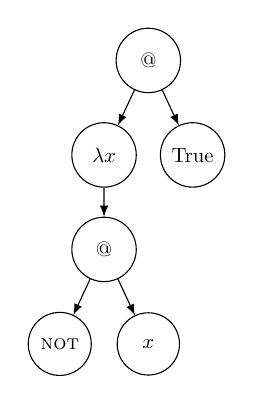
\begin{tikzpicture}[
			scale=0.75, transform shape,
			main/.style = {draw, circle},
			edge from parent/.style={draw,-latex},
			level distance=1.6cm,align=center,text width=0.75cm,
			]
			\node[main] (root) {@}
			child { node[main] {$\lambda x$}
				child { node[main] {@}
					child { node[main] {\textsc{not}} }
					child { node[main] {$x$} }
				}
			}
			child { node[main] {True} };
		\end{tikzpicture}
		\subcaption{Abstraktno sintaksno drevo \textit{pred} redukcijo}
		\label{fig:redukcija-aplikacije-pred}
	\end{subfigure}%
	\hfill
	\begin{subfigure}[b]{0.45\textwidth}
		\centering
		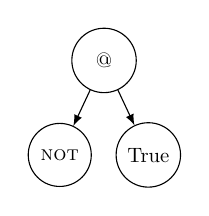
\begin{tikzpicture}[
			scale=0.75, transform shape,
			main/.style = {draw, circle},
			edge from parent/.style={draw,-latex},
			level distance=1.6cm,align=center,text width=0.75cm,
			]
			\node[main] (root) {@}
			child { node[main] {\textsc{not}} }
			child { node[main] {True} };
		\end{tikzpicture}
		\subcaption{Abstraktno sintaksno drevo \textit{po} redukciji}
		\label{fig:redukcija-aplikacije-po}
	\end{subfigure}
	\caption{Redukcija grafa izraza $(\lambda x \, . \, \textsc{not} \; x) \; \texttt{True}$}
	\label{fig:redukcija-aplikacije}
\end{figure*}

Slika \ref{fig:redukcija-dvojne-aplikacije} prikazuje en korak redukcije abstraktnega sintaksnega drevesa izraza $(\lambda x \, . \, \textsc{and} \; x \; x) \; (\textsc{not} \; \texttt{True})$. Po enem koraku redukcije sintaksnega telesa, se \textit{vse uporabe} parametra $x$ zamenjajo z njegovo vrednostjo. Ker je takih pojavitev več, pa rezultat ni več drevo, temveč acikličen usmerjen graf. Na pomnilniku tak izraz predstavimo z dvema kazalcema na isti objekt. Ko se objekt prvič izračuna, se vrednost objekta na pomnilniku posodobi z izračunano vrednostjo. Ob vseh nadaljnjih uporabah argumenta, tako ne bo potrebno še enkrat računati njegove vrednosti, s čemer dosežemo, da bo vsak argument izračunan največ enkrat. 

\begin{figure*}[ht]
	\centering
	\begin{subfigure}[b]{0.45\textwidth}
		\centering
		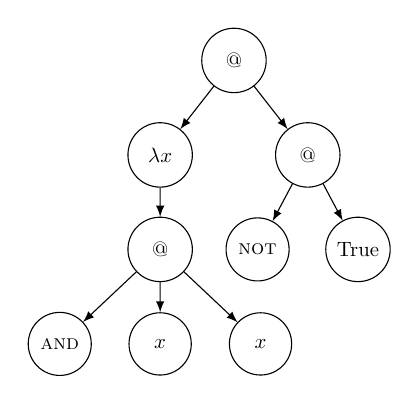
\begin{tikzpicture}[
			scale=0.75, transform shape,
			main/.style = {draw, circle},
			edge from parent/.style={draw,-latex},
			level distance=1.6cm,align=center,text width=0.75cm,
			level 1/.style={sibling distance=2.5cm},
			level 2/.style={sibling distance=1.7cm},
			]
			\node[main] (root) {@}
			child { node[main] {$\lambda x$}
				child { node[main] {@}
					child { node[main] {\textsc{and}} }
					child { node[main] {$x$} }
					child { node[main] {$x$} }
				}
			}
			child { node[main] {@}
				child { node[main] {\textsc{not}} }
				child { node[main] {True} }
			};
		\end{tikzpicture}
	\end{subfigure}%
	\hfill
	\begin{subfigure}[b]{0.45\textwidth}
		\centering
		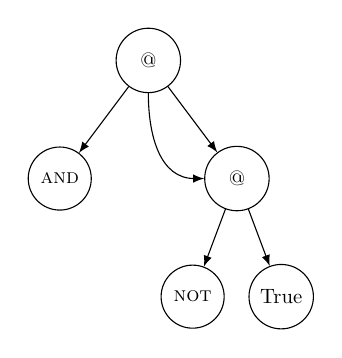
\begin{tikzpicture}[
			scale=0.75, transform shape,
			main/.style = {draw, circle},
			edge from parent/.style={draw,-latex},
			level distance=2cm,align=center,text width=0.75cm,
			]
			\node[main] (root) {@}
			child { node[main] {\textsc{and}} }
			child { edge from parent[draw=none] }
			child { node[main] (argument) {@}
				child { node[main] {\textsc{not}} }
				child { node[main] {True} }
			};
			\draw[-latex] (root) to[out=-90, in=180, looseness=1.1] (argument);
		\end{tikzpicture}
	\end{subfigure}
	\caption{Redukcija grafa izraza $(\lambda x \, . \, \textsc{and} \; x \; x) \; (\textsc{not} \; \texttt{True})$}
	\label{fig:redukcija-dvojne-aplikacije}
\end{figure*}

Slika \ref{fig:funkcija-y} prikazuje dve možni implementaciji ciklične funkcije $Y \; f = f \; (Y \; f)$. Za razliko od primerov na slikah \ref{fig:redukcija-aplikacije} in \ref{fig:redukcija-dvojne-aplikacije}, pri katerih je bilo reducirano sintaktično drevo še vedno usmerjen acikličen graf, pa temu pri funkciji $Y$ ni več tako. Funkcija $Y$ je namreč rekurzivna, kar pomeni, da se sama pojavi kot vrednost svojega argumenta. Na sliki \ref{fig:funkcija-y-kot-prosta-spremenljivka} je funkcija $Y$ implementirana s pomočjo acikličnega grafa, a v svojem telesu vseeno dostopa do proste spremenljivke $Y$, zaradi česar obstaja na pomnilniku cikel. Na sliki \ref{fig:funkcija-y-kot-cikel} je funkcija implementirana neposredno s pomnilniškem ciklu, kjer je vrednost argumenta kar vozlišče samo.

\begin{figure*}[ht]
	\centering
	\begin{subfigure}[b]{0.45\textwidth}
		\centering
		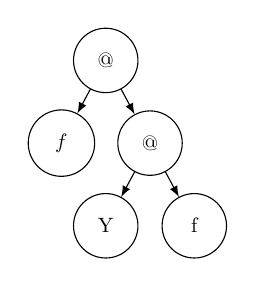
\begin{tikzpicture}[
			scale=0.75, transform shape,
			main/.style = {draw, circle},
			edge from parent/.style={draw,-latex},
			level distance=1.4cm,align=center,text width=0.75cm,
			]
			\node[main] (root) {@}
			child { node[main] {$f$} }
			child { node[main] {@}
				child { node[main] {Y} }
				child { node[main] {f} }
			};
		\end{tikzpicture}
		\subcaption{Funkcija $Y$ implementirana z uporabo proste spremenljivke}
		\label{fig:funkcija-y-kot-prosta-spremenljivka}
	\end{subfigure}%
	\hfill
	\begin{subfigure}[b]{0.45\textwidth}
		\centering
		\begin{tikzpicture}[
			scale=0.75, transform shape,
			main/.style = {draw, circle},
			edge from parent/.style={draw,-latex},
			level distance=1.4cm,align=center,text width=0.75cm,
			]
			\node[main] (root) {@}
			child { node[main] {$f$} }
			child { node (right) {} edge from parent[draw=none] };
			\coordinate [above=0.6cm of root] (above-root);
			\coordinate [right=0.4cm of right] (right-of-right);
			\coordinate (intermediate) at (right-of-right |- above-root);
			\draw[-latex] (root) -- (right.center) -- (right-of-right) -- (intermediate) -- (above-root) -- (root.north);
		\end{tikzpicture}
		\subcaption{Funkcija $Y$ implementirana kot cikličen usmerjen graf}
		\label{fig:funkcija-y-kot-cikel}
	\end{subfigure}
	\caption{Graf funkcije $Y \; f = f \; (Y \; f)$}
	\label{fig:funkcija-y}
\end{figure*}

\subsubsection{Zapis grafa na pomnilniku}

Leni izračun najpogosteje implementiramo s pomočjo zakasnjenih izrazov oziroma zakasnitev (angl. thunks). Te so na pomnilniku predstavljene kot ovojnice, tj. strukture s kazalcem na kodo, ki izračuna njihovo vrednost in polj, ki vsebujejo vezane in proste spremenljivke. Ob izračunu zakasnitve (angl. forcing a thunk) se najprej izračuna njena vrednost, iz\-ra\-ču\-na\-no vrednost, nato pa se izračunana vrednost shrani v strukturo na pomnilniku, da je ob naslednji evalvaciji ni potrebno ponovno računati. Pravimo, da se vrednost na pomnilniku \emph{posodobi}. Tako v programskem jeziku zagotovimo nestrogo semantiko, pri kateri se vsak izraz izračuna \textit{največ enkrat}. Če se argument ne pojavi nikjer v telesu funkcije, se zakasnitve nikoli ne računa, če pa se v telesu pojavi večkrat, se vrednost izračuna enkrat, za vsako nadaljnjo evalvacijo argumenta pa se preprosto vrne vrednost shranjeno na pomnilniku.

Slika \ref{fig:shema-vozlisca-pomnilnik} prikazuje eno izmed možnih predstavitev vozlišča grafa. Sestavljena je iz oznake vozlišča in polj z vsebino oziroma argumenti $a_1, \dots, a_n$.  Oznaka je vrednost, ki predstavlja vrsto vozlišča: aplikacija funkcije, primitivna operacija, celoštevilska vrednost, preusmeritev, ipd. V poglavju \ref{sec:stg-definicija} bomo videli, da sta si struktura \ref{fig:shema-vozlisca-pomnilnik} in pomnilniški zapis objektov v jeziku STG precej podobna.

\begin{figure*}[ht]
	\centering
	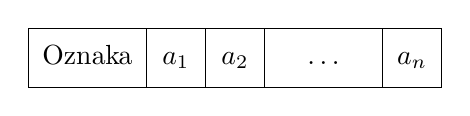
\begin{tikzpicture}[
		% Popravi vertikalno pozicioniranje teksta
		% https://tex.stackexchange.com/a/133237/324113
		verticalalign/.append style={font=\vphantom{Ag}},
		scale=0.75,
		]
		\draw[verticalalign] (0,0) rectangle ++(2,1) node[midway] {Oznaka};
		\draw[verticalalign] (2,0) rectangle ++(1,1) node[midway] {$a_1$};
		\draw[verticalalign] (3,0) rectangle ++(1,1) node[midway] {$a_2$};
		\draw[verticalalign] (4,0) rectangle ++(2,1) node[midway] {$\dots$};
		\draw[verticalalign] (6,0) rectangle ++(1,1) node[midway] {$a_n$};
	\end{tikzpicture}
	\caption{Pomnilniška predstavitev vozlišča grafa}
	\label{fig:shema-vozlisca-pomnilnik}
\end{figure*}

Slika \ref{fig:leni-izracun-pomnilnik-izraz} prikazuje predstavitev izraza $\textsc{and} \; (\textsc{not} \; \texttt{True}) \; (\textsc{not} \; \texttt{True})$ na pomnilniku. Celoten izraz je sestavljen iz dveh ovojnic, ki predstavljata dve aplikaciji. Spodnja ovojnica predstavlja izraz $\textsc{not} \; \texttt{True}$ in je sestavljena kot aplikacija funkcije \textsc{not} na argument z vrednostjo \texttt{0x0001}, tj. vrednost \texttt{True}. Zgornja ovojnica predstavlja aplikacijo funkcije \textsc{and} na dva argumenta, ki sta predstavljena kot kazalca na drugo ovojnico. Ko se izraz $\textsc{not} \; \texttt{True}$ prvič izračuna, se ovojnica na pomnilniku posodobi z iz\-ra\-ču\-na\-no vrednostjo. Pri tem se navadno na pomnilniku ustvari nova struktura, ovojnico pa se prepiše s preusmeritvijo na novonastalo strukturo. Tako ob vseh nadaljnjih dostopih, vrednosti ovojnice ni potrebno ponovno računati.

\begin{figure*}[ht]
	\centering
	\begin{tikzpicture}[scale=0.8]
		\draw (0,0) rectangle ++(1,1) node[midway] {\textbf{@}};
		\draw (1,0) rectangle ++(2,1) node[midway] (and) {};
		\draw (3,0) rectangle ++(2,1) node[midway] (and-arg1) {};
		\draw (5,0) rectangle ++(2,1) node[midway] (and-arg2) {};
		
		\draw (0,-2) rectangle ++(1,1) node[midway] (app-not) {\textbf{@}};
		\draw (1,-2) rectangle ++(2,1) node[midway] (not) {};
		\draw (3,-2) rectangle ++(2,1) node[midway] {\texttt{0x0001}};
		
		\node (above-and) at (2,2) {\textsc{and}};
		\node (below-not) at (2,-3) {\textsc{not}};
		
		\draw[Circle-] (4,0.5) -- ++(0,-1);
		\draw[Circle-Latex] (6,0.5) -- ++(0,-1) -- ++(-7,0) -- ++(0,-1) -- ++(1,0);
		
		\draw[Circle-Latex] (2,0.5) -- ++(0,1);
		\draw[Circle-Latex] (2,-1.5) -- ++(0,-1);
		% \draw[-latex] (and) -- (above-and);
	\end{tikzpicture}
	\caption{Predstavitev izraza $\textsc{and} \; (\textsc{not} \; \texttt{True}) \; (\textsc{not} \; \texttt{True})$ na pomnilniku}
	\label{fig:leni-izracun-pomnilnik-izraz}
\end{figure*}

Ena izmed slabosti jezikov z lenim izračunom je, da je, za razliko od neučakanih imperativnih jezikov, zelo težko predvideti, koliko prostora bo program porabil. Ker so v takih jezikih funkcije navadno obravnavane kot primitivi, kar pomeni, da lahko nastopajo kot vrednost argumenta ali rezultata, je lahko njihovo izvajanje zamaknjeno v čas po koncu izvajanja funkcije, ki je ustvarila vrednost argumenta ali rezultata. Zato klicnih zapisov takih funkcij ni mogoče hraniti na skladu, temveč na kopici~\cite{jones2023garbage}. Pri izvajanju se tako na kopici nenehno ustvarjajo in brišejo nove ovojnice, ki imajo navadno zelo kratko življenjsko dobo, zato je nujna učinkovita implementacija dodeljevanja in sproščanja pomnilnika. Haskell za to uporablja \textit{generacijski} avtomatični čistilec pomnilnika~\cite{sansom1993generational, GHC}. Danes vsi večji funkcijski programski jeziki, ki omogočajo leni izračun, uporabljajo avtomatični čistilec pomnilnika~\cite{turner1985miranda, czaplicki2012elm, brus1987clean, syme2017the, sperber2009revised6}.
% Programski jezik Rust je namenjen nizkonivojskemu programiranju, tj. programiranju sistemske programske opreme. Kot tak mora omogočati hitro in predvidljivo sproščanje pomnilnika, zato avtomatični čistilnik pomnilnika ne pride v poštev. Rust namesto tega implementira model lastništva~\cite{klabnik2023rust}, pri katerem zna med \textit{prevajanjem} s posebnimi pravili zagotoviti, da se pomnilnik objektov na kopici avtomatično sprosti, kadar jih program več ne potrebuje. Po hitrosti delovanja se tako lahko kosa s programskim jezikom C, pri tem pa zagotavlja varnejše upravljanje s pomnilnikom kot C.

Rust doseže varnost pri upravljanju pomnilnika s pomočjo principa izključitve (angl. exclusion
principle)~\cite{jung2020understanding}. V poljubnem trenutku za neko vrednost na pomnilniku velja natanko ena izmed dveh možnosti:

\begin{itemize}
	\itemsep 0em
	\item Vrednost lahko \textit{spreminjamo} preko \textit{natanko enega} unikatnega kazalca
	\item Vrednost lahko \textit{beremo} preko poljubno mnogo kazalcev
\end{itemize}

V nadaljevanju si bomo na primerih ogledali principa premika in izposoje v jeziku Rust. V vseh primerih bomo uporabljali terko \texttt{Complex}, ki predstavlja kompleksno število z dvema celoštevilskima komponentama in je definirana kot \mintinline{rust}{struct Complex(i32, i32)}.

\section{Premik}

Princip lastništva je eden izmed najpomembnejših konceptov v programskem jeziku Rust. Ta zagotavlja, da si vsako vrednost na pomnilniku lasti natanko ena spremenljivka. Ob prirejanju, tj. izrazu \mintinline{rust}|let x = y|, pride do \textit{premika} vrednosti na katero kaže spremenljivka \var{y} v spremenljivko \var{x}. Po prirejanju postane spremenljivka \var{y} neveljavna in se nanjo v nadaljevanju programa ni več moč sklicevati. Kadar gre spremenljivka, ki si lasti vrednost na pomnilniku izven dosega (angl. out-of-scope), lahko tako Rust ustrezno počisti njen pomnilnik. Naslednji primer prikazuje program, ki se v Rustu ne prevede zaradi težav z lastništvom.

\begin{rust-failure}
let number = Complex(0, 1);
let a = number;
let b = number;  // Napaka: use of moved value: `number`
\end{rust-failure}

Spremenljivka \var{a} prevzame lastništvo nad vrednostjo na katero kaže spremenljivka \var{number}, tj. strukturo \mintinline{rust}|Complex(0, 1)|. Ob premiku postane spremenljivka \var{number} neveljavna, zato pri ponovnem premiku v spremenljivko \var{b}, prevajalnik javi napako.

Pravila lastništva~\cite{klabnik2023rust} so v programskem jeziku Rust sledeča:

\begin{itemize}
	\itemsep 0em
	\item Vsaka vrednost ima lastnika.
	\item V vsakem trenutku je lahko lastnik vrednosti le eden.
	\item Kadar gre lastnik izven dosega (angl. out-of-scope), je vrednost spro\-šče\-na.
\end{itemize}

Rustov model lastništva lahko predstavimo tudi kot graf, v katerem vozlišča predstavljajo spremenljivke oziroma objekte na pomnilniku, povezava med vozlišči $u \to v$ pa označuje, da si spremenljivka $u$ lasti spremenljivko $v$. Ker ima vsaka vrednost natanko enega lastnika, lahko sklepamo, da je tak graf ravno drevo. Kadar gre spremenljivka $v$ izven dosega, lahko Rust počisti celotno poddrevo s korenom $v$ tako, da rekurzivno sprosti pomnilnik za spremenljivke, ki si jih vozlišče $v$ lasti, nato pa počisti še svoj pomnilnik. Preverjanje veljavnost pravil poteka v fazi analize premikov (angl. move check), v program pa se v tej fazi na ustrezna mesta dodajo tudi ukazi za sproščanje pomnilnika.

\subsection{Prenos lastništva pri klicu funkcije}

Kadar je spremenljivka uporabljena v argumentu pri klicu funkcije, je vrednost spremenljivke premaknjena v funkcijo. Če se vrednost spremenljivke uporabi za sestavljanje rezultata funkcije, potem je vrednost ponovno premaknjena iz funkcije in vrnjena klicatelju. Naslednji primer prikazuje identiteto implementirano v Rustu. Pri klicu funkcije, je vrednost spremenljivke \var{number} premaknjena v klicano funkcijo, ker pa je ta uporabljena pri rezultatu funkcije, je vrednost ponovno premaknjena v spremenljivko \var{a} v klicatelju.

\begin{rust-success}
fn identiteta(x: Complex) -> Complex { x }
let number = Complex(0, 1);
let a = identiteta(number);
\end{rust-success}

V naslednjem primeru funkcija \var{prepisi} prevzame lastništvo nad vrednostjo \mintinline{rust}|Complex(0, 1)|, vrne pa novo vrednost \mintinline{rust}|Complex(2, 1)|, pri čemer ne uporabi argumenta funkcije. Funkcija \var{prepisi} je tako odgovorna za čiščenje pomnilnika vrednosti argumenta \var{x}.

\begin{rust-success}
fn prepisi(x: Complex) -> Complex { Complex(2, 1) }
let number = Complex(0, 1);
let a = prepisi(number);
\end{rust-success}

\section{Izposoja}

Drugi koncept, ki ga definira Rust je \textit{izposoja}. Ta omogoča \textit{deljenje} (angl. aliasing) vrednosti na pomnilniku. Izposoje so lahko spremenljive (angl. mutable) \texttt{\&mut x} ali nespremenljive (angl. immutable) \texttt{\&x}. Po principu izključitve, je lahko v danem trenutku ena spremenljivka izposojena nespremenljivo oziroma samo za branje (angl. read-only) večkrat, spremenljivo pa natanko enkrat. Preverjanje veljavnosti premikov se v Rustu izvaja v fazi analize izposoj (angl. borrow check), v kateri se zagotovi, da reference ne živijo dlje od vrednosti na katero se sklicujejo, prav tako pa poskrbi, da je lahko vrednost ali izposojena enkrat spremenljivo ali da so vse izposoje nespremenljive.

Naslednji primer se v Rustu uspešno prevede, ker sta obe izposoji nespremenljivi. Vrednosti spremenljivk \var{a} in \var{b} lahko le beremo, ne moremo pa jih spreminjati. Prav tako je prepovedano spreminjati vrednost spremenljivke \var{number}, dokler nanjo obstaja aktivna izposoja. 

\begin{rust-success}
let number = Complex(2, 1);
let a = &number;
let b = &number;
\end{rust-success}

Zaradi principa izključitve je v Rustu prepovedano ustvariti več kot eno spremenljivo referenco na objekt. V primeru, da bi bilo dovoljeno ustvariti več spremenljivih referenc, bi namreč lahko več niti hkrati spreminjalo in bralo vrednost spremenljivke, kar krši pravila varnosti pomnilnika, saj lahko privede do \komentar{tveganih stanj} (angl. data races). V naslednjem primeru skušamo ustvariti dve spremenljivi referenci, zaradi česar prevajalnik ustrezno javi napako.

\begin{rust-failure}
let mut number = Complex(1, 2);
let a = &mut number;
let b = &mut number;  // Napaka: cannot borrow `number` as mutable
                      // more than once at a time
\end{rust-failure}

Prav tako v Rustu ni veljavno ustvariti spremenljive reference na spremenljivko, dokler nanjo obstaja kakršnakoli druga referenca. V nasprotnem primeru bi lahko bila vrednost v eni niti spremenjena, medtem ko bi jo druga nit brala.

\begin{rust-failure}
let mut number = Complex(0, 0);
let a = &number;
let b = &mut number;  // Napaka: cannot borrow `number` as mutable
                      // because it is also borrowed as immutable
\end{rust-failure}

%\subsubsection{Ponovna izposoja}
%
%\begin{rust-success}
%let number = Complex(2, 1);
%let a = &number;
%let b = *a;
%\end{rust-success}

\subsection{Življenjske dobe}

Kot smo že omenili, analiza izposoj v Rustu zagotovi, da v danem trenutku na eno vrednost kaže le ena spremenljiva referenca ali da so vse reference nanjo nespremenljive. Prav tako pa mora prevajalnik v tej fazi zagotoviti, da nobena referenca ne živi dlje od vrednosti, ki si jo izposoja. To doseže z uvedbo \textit{življenjskih dob} (angl. lifetimes), ki predstavljajo časovne okvirje, v katerih so reference veljavne. Prevajalnik navadno življenjske dobe določi implicitno s pomočjo dosegov (angl. scopes). Vsak ugnezden doseg uvede novo življenjsko dobo, za katero velja, da živi največ tako dolgo kot starševski doseg. Kadar se namreč izvedejo vsi stavki v dosegu, bo pomnilnik vseh spremenljivk, definiranih v dosegu, sproščen. Življenjske dobe označujemo z oznakami \texttt{'a}, \texttt{'b}, \dots, najdaljša življenjska doba pa nosi oznako \texttt{'static}, ki označuje, da je objekt živ tekom celotnega izvajanja programa.

\begin{rust-failure}
let outer;
{
    let inner = 3;
    outer = &inner;  // Napaka: `inner` does not live
                     // long enough
}
\end{rust-failure}

Zgornji primer prikazuje program, ki se v Rustu ne prevede zaradi težav z življenjskimi dobami. Program je sestavljen iz dveh dosegov:
\begin{itemize}
	\itemsep 0em
	\item Spremenljivka \var{outer} živi v zunanjem dosegu, prevajalnik ji dodeli živ\-ljen\-jsko dobo \texttt{'a}.
	\item Nov blok povzroči uvedbo novega dosega z živ\-ljenj\-sko dobo \texttt{'b}, zato prevajalnik spremenljivki \var{inner} določi živ\-ljenj\-sko dobo \texttt{'b}.
\end{itemize}

Ker je notranji doseg uveden znotraj zunanjega dosega, si prevajalnik tudi označi, da je življenjska doba \texttt{'a} vsaj tako dolga kot doba \texttt{'b} (oziroma da mora biti življenjska doba \texttt{'b} največ tako dolga kot \texttt{'a}). To pomeni, da bodo vse spremenljivke, ki so definirane znotraj notranjega dosega živele manj časa od spremenljivk definiranih v zunanjem dosegu. Rust počisti pomnilnik spremenljivke \var{inner}, kadar se notranji doseg konča. V našem primeru bi tako spremenljivka \var{outer} kazala na spremenljivko, ki je že bila uničena, s čemer pa bi v program uvedli viseč kazalec, kar pa krši varnostni model jezika, zato v tem primeru Rust vrne napako.

\subsection{Eksplicitno navajanje življenjskih dob}

V Rustu so eksplicitne življenjske dobe potrebne, kadar prevajalnik ne more samodejno določiti razmerij med življenjskimi dobami referenc v podpisih funkcij, metod ali struktur. Do tega pride pri funkcijah, ki sprejmejo več argumentov in vrnejo rezultat, ki se sklicuje na nekatere izmed njih ali pri strukturah, ki v poljih vsebujejo reference. V teh primerih mora Rust zagotoviti, da so vrnjene reference veljavne vsaj tako dolgo, kot je potrebno, česar pa ne zna izpeljati avtomatično, zato mora programer navesti življenjske dobe eksplicitno.

Naslednji primer prikazuje program, pri katerem pride do napake zaradi nepravilno definiranih življenjskih dob.  Funkcija \var{longest} vrne referenco na daljšo besedo. Po definiciji ta sprejme dve referenci z \emph{enako} življenjsko dobo \texttt{'a} in vrne referenco z življenjsko dobo \texttt{'a}, ki živi tako dolgo kot oba argumenta. V funkciji \var{main}, so definirane tri spremenljivke: \var{first} in \var{result} sta deklarirani v istem bloku in imata zato enako življenjsko dobo, spremenljivka \var{second} pa je deklarirana v ugnezdenem bloku in ima tako krajšo življenjsko dobo. Kadar se notranji blok zaključi, se počisti tudi pomnilnik spremenljivke \var{second}. Toda, v spremenljivko \var{result} se shrani kazalec na daljšo izmed besed, kar je v našem primeru spremenljivka \var{second}, ki pa je izbrisana preden se rezultat izpiše na ekran. Rust zna s pomočjo eksplicitno navedenih življenjskih dob napako tudi odkriti in vrniti napako.

\begin{rust-failure}
fn longest<'a>(first: &'a str, second: &'a str) -> &'a str;
fn main() {
    let first = String::from("Rust");
    let result;
    {
        let second = String::from("Haskell");
        result = longest(first.as_str(), second.as_str());
        // Spremenljivka 'second' gre tukaj izven dosega
    }
    println!("{}", result);
}
\end{rust-failure}

V določenih preprostih primerih zna Rust izpeljati življenjske dobe sam. Predvsem zaradi pisanja krajše kode, Rust namreč podpira izpuščanje živ\-ljenj\-skih dob (angl. lifetime elision) v določenih primerih. Pri tej na podlagi treh pravil prevajalnik samodejno ustvari oziroma dopolni življenjske dobe vhodnih in izhodnih argumentov. Če npr. funkcija kot vhod sprejme referenco in vrne referenco, prevajalnik predpostavlja, da imata obe enaki življenjski dobi. Kadar prevajalnik po pravilih življenjskih dob ne zna izpeljati, prevajalnik vrne napako, odgovornost za eksplicitno navajanje živ\-ljenj\-skih dob pa preda programerju. 

\begin{rust-success}
fn id(x: &i32) -> &i32;
fn id<'a>(x: &'a i32) -> &'a i32;
\end{rust-success}

\subsection{Opombe}
% Non-lexical lifetimes
Od leta 2022 Rust podpira neleksikalne življenjske dobe (angl. non-lexical lifetimes)~\cite{Matsakis_2018, Matsakis_et_al_2022}, pri katerih se preverjanje izposoj in premikov izvaja nad grafom poteka programa (angl. control flow graph) namesto nad abstraktnim sintaktičnim drevesom programa~\cite{weiss2021oxide, StackedBorrows}. Prevajalnik zna s pomočjo neleksikalnih življenjskih dob dokazati, da sta dve zaporedni spremenljivi izposoji varni, če ena izmed njih ni nikjer uporabljena. Na tak način Rust zagotovi bolj drobnozrnat (angl. fine grained) pogled na program, saj prevajalnik vrača napake ob manj veljavnih programih.

Potrebno je poudariti, da bi se vsi primeri v tem poglavju v trenutni različici Rusta zaradi neleksikalnih življenjskih dob vseeno prevedli. Primere smo namreč zaradi boljšega razumevanja in jedrnatosti prikaza nekoliko poenostavili. Ker deklarirane spremenljivke nikjer v prihodnosti niso več uporabljene, zna Rust z analizo živosti prepoznati, da sta npr. dve zaporedni spremenljvi izposoji varni, saj vrednost ni nikoli več spremenjena. Zato za vse primere v tem poglavju predpostavljamo, da so tako premaknjene, kot tudi izposojene spremenljivke v nadaljevanju programa še nekje uporabljene.

\subsection{Sorodno delo}
% Formalizacije Rusta
Kljub temu, da Rust v svoji dokumentaciji~\cite{klabnik2023rust} zagotavlja, da je njegov model upravljanja s pomnilnika varen, pa njegovi razvijalci niso nikoli uradno formalizirali niti njegove operacijske semantike, niti sistema tipov, niti modela za prekrivanje (angl. aliasing model). V literaturi se je tako neodvisno uveljavilo več modelov, ki skušajo čimbolj natančno formalizirati semantiko premikov in izposoj. Model Patina~\cite{reed2015patina} formalizira delovanje analize izposoj v Rustu in dokaže, da velja izrek o varnosti (angl. soundness) za varno (angl. safe) podmnožico jezika Rust. Model RustBelt~\cite{10.1145/3158154} poda prvi formalen in strojno preverjen dokaz o varnosti za jezik, ki predstavlja realistično podmnožico jezika Rust. Model Stacked borrows~\cite{StackedBorrows} definira operacijsko semantiko za dostopanje do pomnilnika v Rustu in model za prekrivanje (angl. aliasing model) in ga strojno dokaže. Model Oxide~\cite{weiss2021oxide} je formalizacija Rustovega sistema tipov in je tudi prva semantika, ki podpira tudi neleksikalne življenjske dobe. 